\chapter{Chrome擴充套件設計與實作}
\indent
在撰寫網頁測試腳本時,
為了避免網頁改版後,腳本內部中專門定位內部元件的Xpath無法正確抓取元件位置導致腳本頻頻出錯,
需要提高專門定位網頁中元件Xpath表達式的穩定性。

本論文以呂昭陞"提出提升穩定性的Xpath撰寫樣式"論文中的觀念為基礎,尋找符合的限制條件並建立一個穩定性高的網頁測試腳本,
但對於需要找出好的限制條件,對測試人員會是需要一定的經驗且較花時間的事情。
因此本論文提出在測試人員需要找尋適合的條件的時候可以透過Chrome擴充套件增加比較HTML文檔和過濾自訂屬性...等等額外功能的設計,
讓使用者即使在大型架構的HTML中也可以減少對於測試人員屬於雜訊的元件,可以較快速的挑選出想要屬性來設定適合的條件,
來撰寫適合定位該元件的Xpath表達式。

% =========================================================================================
% =========================================================================================
\section{擴充元件之使用情境}\label{s3.1}

在章節\ref{s2.4}有提到Xpath的組成方式,分別是Axis、Node test和零個或多個Predicate。
為了確保表達式中的穩定性,通常在設計時,都會同時使用這三種原件來組成一個路徑表達式。

在撰寫測試腳本時,每做完一個元件互動後,通常都需要驗證有相互關係的元件有出現或消失以確保該元件互動有確實被執行,
這時可以利用元件屬性的變化或元件的增減來當Xpath的限制條件,若畫面沒有執行該變化,代表利用此Xpath無法定位該元件,程式會將會執行失敗。
換句話說,若使用者要用一段Xpath表達式來判斷他是否有互動成功,必須要先找出它有哪些變化並加入在Xpath的條件中,
以圖\ref{f3.1}舉例,點擊了按鈕後,
HTML文本中會發現div元件中的class會從"status-one"變成"status-two",
若要用一段xpath表達式來確保有點擊按鈕,
可以撰寫成\colorbox{lightgray}{//div[@class="status-two"]//p[text()="Status msg"]},
如果網頁有問題,互動後元件中的class屬性沒有改變的話,上述Xpath中\colorbox{lightgray}{@class="status-two"}的條件會無法符合,
即無法定位到該元件位置,導致測試腳本執行失敗。

\begin{figure}[H]
    \centering
    \includegraphics[width=0.6\textwidth]{picture/ch3-html-after-change.png}
    \caption{互動後HTML文本改變之範例圖}
    \label{f3.1}
\end{figure}

由上述例子可知,HTML變化後的元件或屬性很適合在測試腳本中當作互動是否成功的判斷。
一般使用者需要查看當下網頁中HTML會打開瀏覽器中的Developer Tools,
藉由Developer Tools中"Inspect Element"的功能,直接跳轉到點選物件的位置來查看元件的變化。
使用者在尋找元件變化的時候,常常會遇到以下兩種變化:

\begin{itemize}
    \item\textbf{元件互動時HTML文本快速變化}

    使用者在網頁中元件有互動行為的時候,
    可以在Developer Tools中觀察HTML文本因為互動而使元件內容或屬性產生快速的變化,
    如圖\ref{f3.2}所示,變化的元件會有紫色的漸淡背景框來提醒使用者。
    通常在元件屬性比較冗長複雜的情況下,
    元件的快速變化會造成使用者可能無法立即觀察出變化,
    需要花較多的時間重複元件互動行為來判斷它其中的差異。

    \begin{figure}[H]
        \centering
        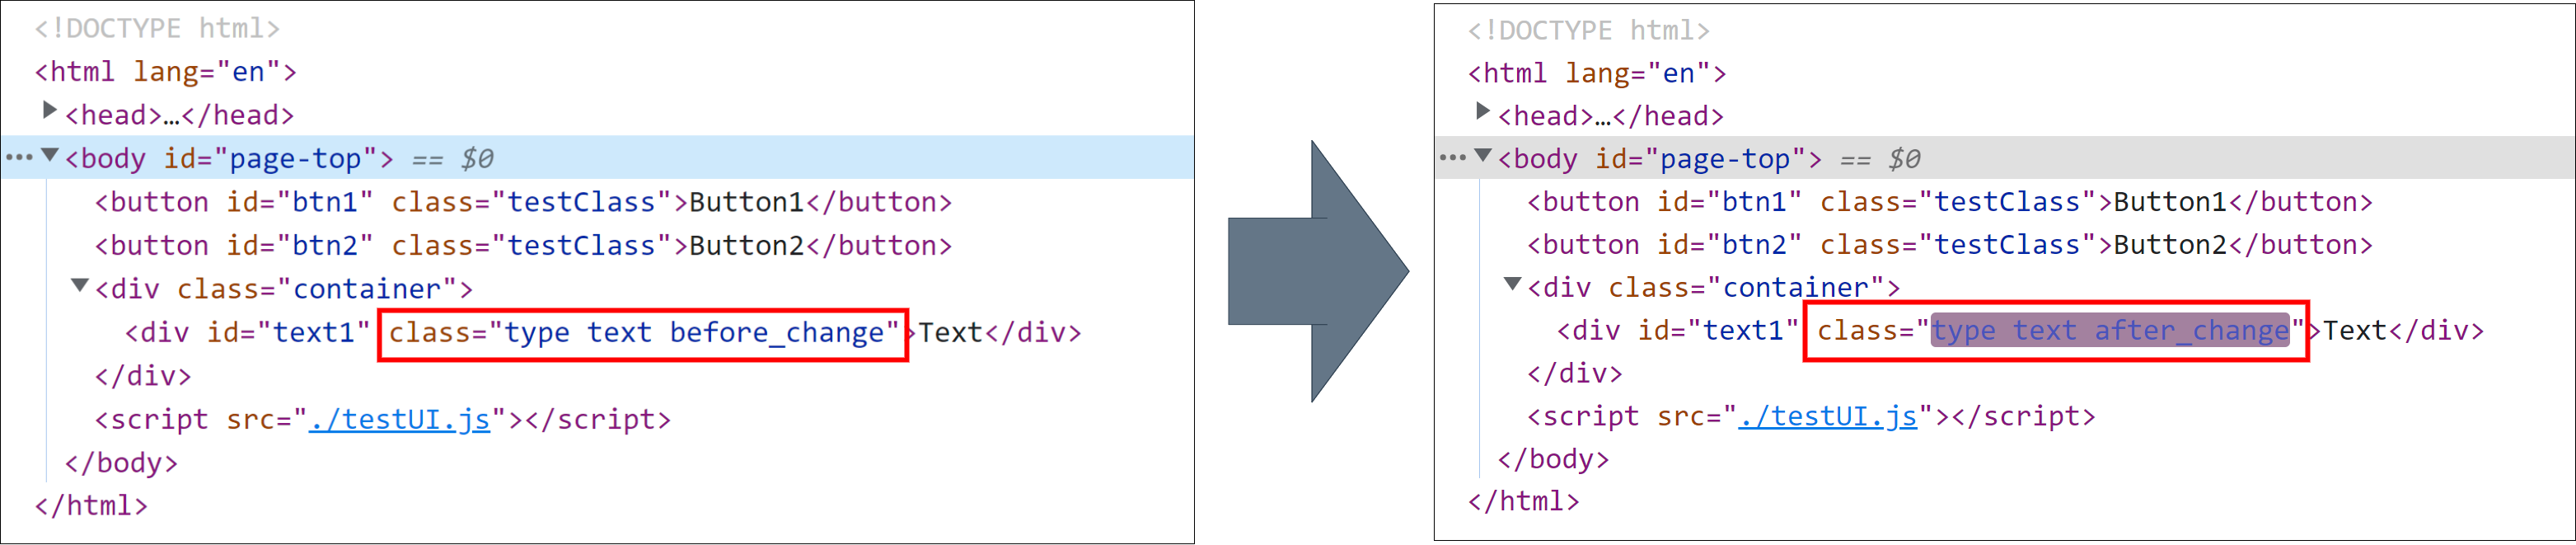
\includegraphics[width=1.0\textwidth]{picture/ch3-element-change-fast.png}
        \caption{HTML互動後元件變化之顯示}
        \label{f3.2}
    \end{figure}
    
    \item\textbf{HTML文本未展開無變化提示}

    通常使用者會利用Developer Tools中"Inspect Element"的功能來找出元件在HTML中的位置,
    在使用這個功能時,會自動展開該元件上層的所有直屬元件,
    因為它只會幫你展開直屬元件,
    若未展開的元件或在Developer Tool中Element頁面需要滾動才看的元件有變化的話,
    較容易會被使用者忽略,
    以圖\ref{f3.3}為例,
    左半部的圖是未展開的狀態,在未展開時,紅色框內的元件並沒有紫色的漸淡背景框,
    若和右半部的圖一樣把元件展開後,才能發現裡面元件的變化並有紫色的漸淡背景框來提示使用者。

    \begin{figure}[H]
        \centering
        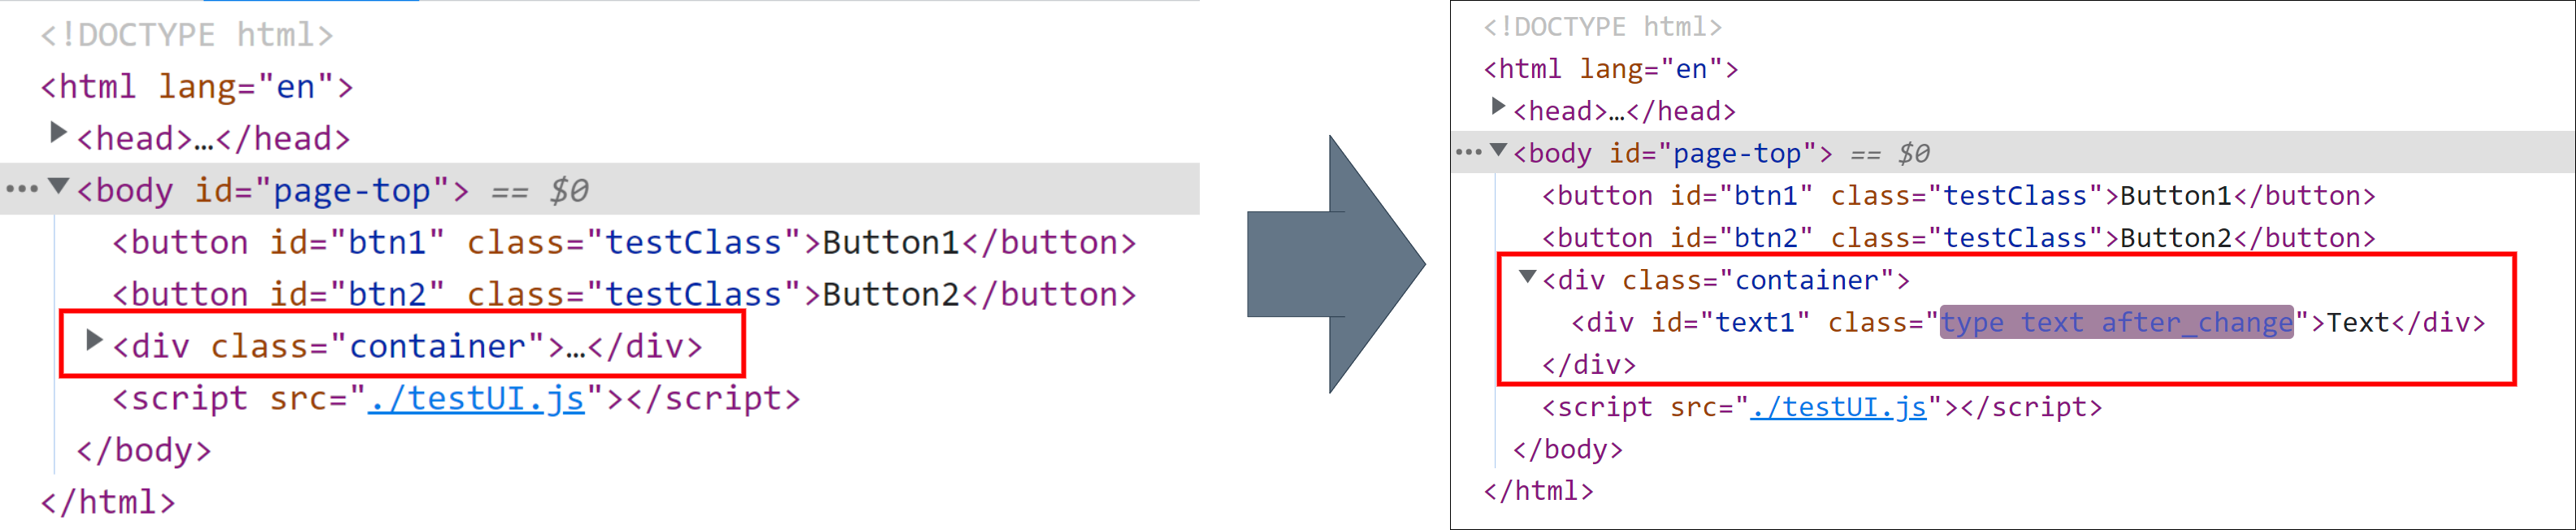
\includegraphics[width=1.0\textwidth]{picture/ch3-element-change-nghide.png}
        \caption{HTML文本未展開導致不會顯示變化提示}
        \label{f3.3}
    \end{figure}
    
\end{itemize}

因為上述兩種原因,會導致找出變化會花較多時間,
在此情況下可以使用此工具利用文本比較的方式把HTML中相異的地方列出,
讓測試人員可以使用工具所列出的差異來設計Xpath,來避免忽略掉較難找出的變化。

% =========================================================================================
% =========================================================================================
\section{系統架構}\label{s3.2}
圖\ref{f3.4}為Chrome擴充套件實作的系統架構圖,下列為各元件之介紹:

\begin{itemize}
\item\textbf{Chrome:}
以市占率第一的Chrome瀏覽器為背景下,對瀏覽器擴充元件進行實作

\item\textbf{Chrome Extension:}
對Chrome瀏覽器加裝此擴充功能之擴充程式

\item\textbf{Background Script For Extension:}
擴充程腳本之一, 屬於擴充元件的背景程序,通常會將程式的主要邏輯放在此腳本中

\item\textbf{SidePanel Script For Extension:}
擴充程式腳本之一, 在擴充元件Element頁面下的子頁面

\item\textbf{HTML Compare Function:}
比對兩個HTML差異之程式模組

\item\textbf{UI Interface:}
擴充元件在SidePanel裡面的使用者介面設計

\item\textbf{Test Script:}
針對Compare Function的單位測試腳本

\end{itemize}

\begin{figure}[H]
    \centering
    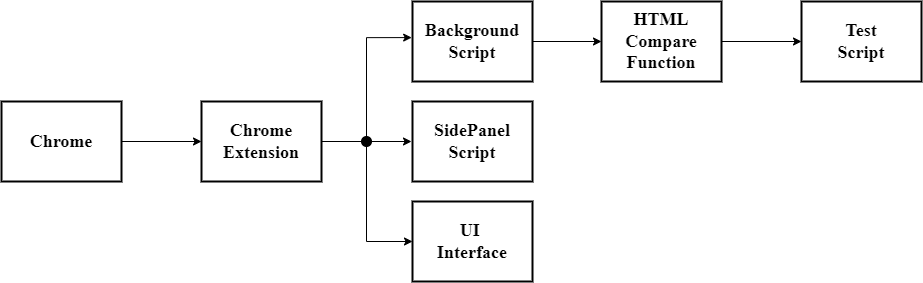
\includegraphics[width=0.9\textwidth]{picture/ch3-systemStucture.png}
    \caption{擴充元件實作之架構圖}
    \label{f3.4}
\end{figure}

此設計架構主要是以HTML比對函數為主,利用Chrome Extension的專用腳本們,把網頁的HTML讀取後丟入該比對系統,
比對完再進行回傳動作,最後利用UI介面把結果顯示在畫面上。

% =========================================================================================
% =========================================================================================
\section{HTML比對之實作}\label{s3.3}
若確定要開始進行比對網頁中的HTML文本後,需要先取出先前和之後的兩個HTML文本,然後進行文本前後比對\cite{HTML-Comparison-Algorithm}。
此比對功能,使用了開源程式Hiff的架構,經過權重部分修改、輸出元件的調整以及增加相關測試腳本,
調整成適合擴充程式的內部核心程式,並將此實作放入擴充程式的Background Script中。圖\ref{f3.5}為HTML比對之活動圖。

\begin{figure}[H]
    \centering
    \includegraphics[width=1.0\textwidth]{picture/ch3-activity diagram.png}
    \caption{HTML比對之活動圖}
    \label{f3.5}
\end{figure}

\subsection{判斷節點相異程度}\label{s3.3.1}
在兩節點相互比對後,需要有一個判斷方法來確定該節點的相異程度,會分成三個等級:Identical、Same but different和Not the same node。
本程式的實作流程為圖\ref{f3.6},會先做比各屬性的比對,然後根據當前狀況選擇要該屬性自定義的權重,最後將所有權重相加來節點判斷相異等級

\begin{figure}[H]
    \centering
    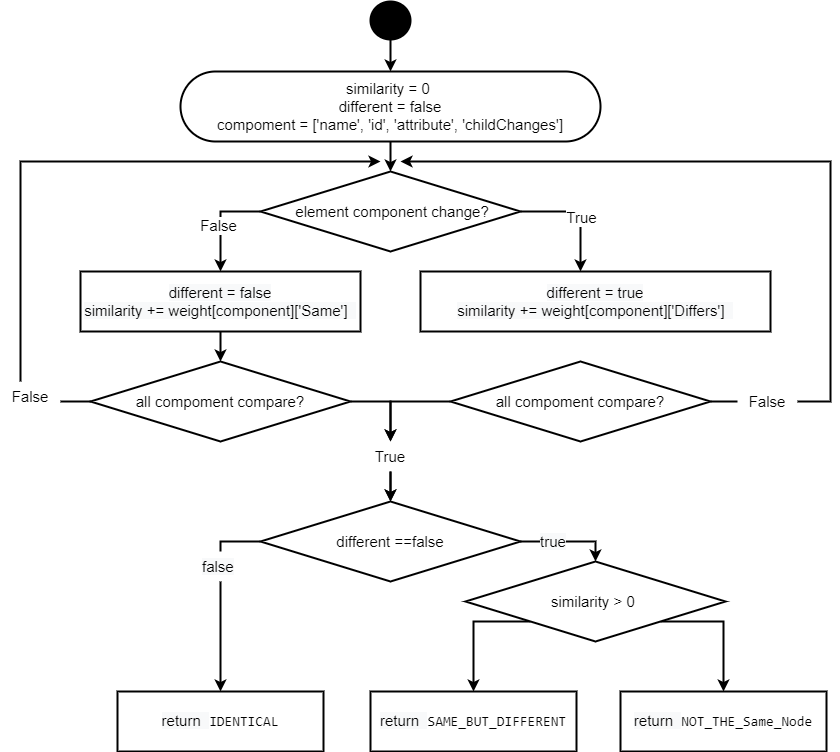
\includegraphics[width=1.0\textwidth]{picture/ch3-HEURISTIC-comapre.png}
    \caption{節點相異程度之活動圖}
    \label{f3.6}
\end{figure}

\subsection{比對輸出結果}\label{s3.3.2}
在比對的時候有分成三種類型:Changed、Added和Removed,三種類型需要回傳相對應的資訊,
舊有的開源程式碼僅只有對該變更資訊用最低限度的字串來表示變更,經過修改後,將輸出結果加上變更節點的解析結果以及詳細屬性變化資訊,
在顯示上可以將結果直接輸出在畫面上,減少其他額外的處理。

在程式碼\ref{l3.1}為changed類型的輸出結果,
其中除了回傳相關的解析後的節點資訊,
裡面"info-compare"的值為比對該變化元件的所有類別結果,包括比對前、比對後和差異結果。

\begin{lstlisting}[caption=比對輸出結果(changed類型), label={l3.1}]
    1   function changed($nodeBefore, $nodeAfter) 
    2   {
    3    var before = grabParentAndIndex($nodeBefore),
    4    after = grabParentAndIndex($nodeAfter);
    5
    6    return {
    7    type: "changed",
    8    before:locationInfo(before.$parent, $nodeBefore, before.index),
    9    after: locationInfo(after.$parent, $nodeAfter, after.index),
    10   selectingNode: $nodeAfter,
    11   nodeINFO: $nodeBefore,
    12   info-compare: info_compare ($nodeBefore, $nodeAfter)
    13   };
    14  }
\end{lstlisting}

在程式碼\ref{l3.2}和程式碼\ref{l3.3}為added和changed類型的輸出結果,
其中除了回傳相關的解析後的節點資訊,
裡面"contentHTML"的值為added或removed元件的內部HTML資訊,會在UI介面中將整個變更的區塊告訴使用者。

\begin{lstlisting}[caption=比對輸出結果(added類型), label={l3.2}]
    1   function added($addedNode, $parentBefore, indexBefore, 
    2       $parentAfter, indexAfter) 
    3   {
    4     return {
    5     type: "added",
    6     before: locationInfo($parentBefore, undefined, indexBefore),
    7     after:  locationInfo($parentAfter, $addedNode, indexAfter),
    8     selectingNode: $parentAfter,
    9     nodeINFO: $addedNode,
    10    contentHTML: stringify($addedNode, false),
    11    };
    12  }
\end{lstlisting}

\begin{lstlisting}[caption=比對輸出結果(removed類型), label={l3.3}]
    1   function removed($removedNode, $parentBefore, indexBefore, 
    2       $parentAfter, indexAfter) 
    3   {
    4    return {
    5    type: "removed",
    6    before: locationInfo($parentBefore, $removedNode, indexBefore),
    7    after:  locationInfo($parentAfter, undefined, indexAfter),
    8    selectingNode: $parentAfter,
    9    nodeINFO: $removedNode,
    10   contentHTML: stringify($removedNode, false),
    11   };
    12  }
\end{lstlisting}


% =========================================================================================
% =========================================================================================
\section{擴充元件腳本設計之實作}\label{s3.4}
\indent
在章節\ref{s2.6.3}有對不同類型的腳本做基本介紹,針對各腳本獨特的特性分配它需要執行的功能。
圖\ref{f3.7}中表示出執行功能後的執行順序及流程,從按下比對文本的按鈕到比對結束的內部腳本們的流程圖。

\indent

\begin{figure}[H]
    \centering
    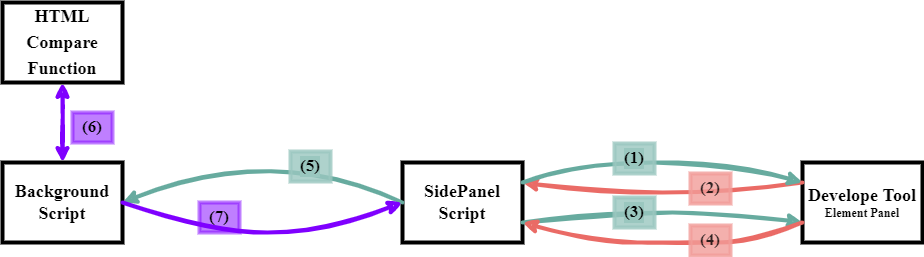
\includegraphics[width=1\textwidth]{picture/ch3-script-structure.png}
    \caption{擴充腳本之溝通順序圖}
    \label{f3.7}
\end{figure}

\subsection{SidePanel Script}\label{s3.4.1}
SidePanel Script是專門控制在Chrome Developer tools中Elements頁面中旁邊子介面的腳本,
此腳本主要功能在於若使用者點擊畫面中的互動按鈕或輸入相關字元,會讓擴充元件開始做動。
在UI介面下點擊開始比對的按鈕後,
等待第一個計時器結束後從Develope Tool中Elements頁面取出當下的HTML文本,
等待第二個計時器結束後再從Develope Tool中Elements頁面取出當下的HTML文本,
共取出變更前以及變更後的兩個HTML文本。
得到兩個文本後,便開始與Background Script溝通讓它知道要開始要進行比對了,
等到比對完後從Background Script得到結果並且把結果回傳給SidePanel Script,
最後將結果顯示在UI介面上,
如圖\ref{f3.7}中的(1)、(2)、(3)、(4)所示。

\subsection{Background Script}\label{s3.4.2}
Background Script在擴充元件中的定位是在背景中執行的程式,開發者通常將此程式的主要邏輯撰寫在這腳本中,
而HTML比對腳本的函數也是在此腳本中執行的,
接收到從SidePanel Script傳來的兩個HTML文本後便會開始比對,
比對後會將最後的比對結果回傳到SidePanel Script中,
如圖\ref{f3.7}中的(5)、(6)、(7)所示。


\section{UI/UX介面之實作}\label{s3.5}
設計此工具,為考慮人性化的使用介面以及比對後的結果方便使用者挑選所需要的條件,將此工具分成以下五個部分:
\begin{itemize}
    \item\textbf{Illustrate:}
    
    說明此擴充工具功能並且敘述該工具選擇的設定方式以及使用流程。

    \item\textbf{Timer:}
    
    依照使用者當前的網路狀況、元件互動情況...等等因素,藉由調整以下兩個Timer來調整抓取HTML文本的時間,

    \begin{itemize}
        \item\textbf{Time Of Set Up}
        
        在點擊"Start Compare"後,此Timer開始倒數計時,等到時間到後,便會抓取第一次的HTML文本。
        此Timer設計是為了讓使用者自定義一個充足的時間設定開始的狀態,讓使用者可以保持一個可控制的環境。
        例如:使用者想要抓取元件原本是Hover狀態到沒有Hover狀態的變化過程,
        可以設定此Timer,讓使用者可以在點擊按鈕後有充足的時間將滑鼠Hover到該元件上。

        \item\textbf{Time Of Change Element}
        
        等"Time Of Set Up"的時間結束並抓取第一次的HTML文本後,
        此Timer開始倒數計時,等到時間到後,
        便會將兩次的HTML文本一同傳送給Background Script執行比對。
 
    \end{itemize}
    
    \item\textbf{Options:}
    
    針對當前使用者狀態,透過選擇對應狀況的選項,讓使用者可以過濾掉大多數不需要的結果

    \begin{itemize}
        \item\textbf{Ignore style attribute's change}
 
        在HTML文件樣式中,有時會利用<style>標籤來建立簡易的CSS指令,但通常在使用時,較少用此標籤來設定條件,
        為避免有很多節點因為style屬性變化,造成比對結果較多不必要的資訊,故設立此條件來篩選。

        \item\textbf{Only display change of current selecting elemnt}
        
        若當前的HTML文本結構過大,但使用者僅僅只是要查看當前節點的變化,過多的變更結果會讓使用者較難找到適合當下情況的條件,
        為過濾掉當前節點之外的變更雜訊,在Develope Tool中Element頁面點擊HTML的節點,比較後的顯示結果僅會出現該節點的變化結果。
        
        \item\textbf{Display one tag's change}
        
        為避免比較後的結果過多,故添加了過濾元件tag的選項,
        讓使用者可以利用節點的tag過濾比對後的結果,例如:div、button...等等類別。

    \end{itemize}
    
    \item\textbf{Compare Control:}
 
    內部有兩個按鈕以及顯示比較情況的顯示框,可以點擊按鈕開始比對或點擊按鈕強制停止比對
    
    \item\textbf{Compare Result:}

    此面板中的下拉選單有顯示三中累行的結果:changed-area、added-area和removed-area,點擊後會出現表格顯示該節點的屬性比對,
    內部表格顯示該節點所有屬性的before、after和diff比對結果
    
    \end{itemize}
\indent

\begin{figure}[H]
    \centering
    \includegraphics[width=1\textwidth]{picture/ch3-UIUX-example.png}
    \caption{UI設計之介面}
    \label{f3.8}
\end{figure}